\documentclass[a4paper]{report}
\usepackage{amsmath,amssymb,booktabs,bm,caption,enumerate,float,geometry,graphicx,hanging,indentfirst,makecell,multirow,setspace,titlesec}
\geometry{left=4.5cm,right=4.5cm,top=4cm,bottom=4cm}
\captionsetup[figure]{labelsep=period}
\captionsetup[table]{labelsep=period}
\begin{document}
\renewcommand\thesection{\arabic{section}}
\begin{Large}
	\begin{center}
		\setlength{\baselineskip}{14pt}
		\vspace{1.25cm}
		\rule[0cm]{11.2cm}{0.03em}\\
		\vspace{0.5cm}
		\textsc{UM-SJTU Joint Institute}\\
		\vspace{0.25cm}
		\textsc{Intro to circuits\\(VE215)}
		\vspace{0.3cm}
		\rule[0cm]{11.8cm}{0.05em}
		\vspace{4.9cm}\\
		\textsc{Laboratory Report}
	\end{center}
\end{Large}
\vspace{0.85cm}
\begin{large}
	\begin{center}
		\textsc{Lab 4}
		\vspace{1em}\\
		\textsc{AC Lab}
	\end{center}
	\vspace{6cm}
\end{large}
\begin{tabular}{l l}
	Name: Yihua Liu&ID: 518021910998\\
	Name: Han Fang&ID: 518370910009\\
	Name: Yiteng Cai&ID: 518370910007\\
	&\\
	Date: \today&\\
\end{tabular}
\thispagestyle{empty}
\newpage
\section{Goal}
\begin{enumerate}
\item
Learn about four types of filters – Low-Pass, High-Pass, Band-Pass, and Band-reject.
\item
Learn about transfer functions.
\item
Predict the theoretical result and make comparison with lab data.
\end{enumerate}
\section{Introduction}
\subsection{Filter}
Filters are everywhere in our lives. The circuits built to operate on signals usually apply filters. For example, telephone lines pass the sounds at frequencies between about 100Hz and 3kHz and practically blocks all other frequencies.
\subsection{Transfer function}
Mathematically, the transfer function is used to analyze what the circuit did to the signal:
$$\rm Transfer\ function=\frac{Output\ signal}{Input\ signal}$$
This function can also be expressed as
$$H(\omega)=\frac{V_{out}(\omega)}{V_{in}(\omega)}$$
The magnitude of the transfer function is called “voltage gain”, often measured as the ratio of the peak-to-peak (ppk) voltages:
$$|H(\omega)|=\left|\frac{V_{out}(\omega)}{V_{in}(\omega)}\right|=\frac{V_{out, ppk}(\omega)}{V_{in, ppk}(\omega)}$$
It is convenient to express and plot the magnitude of the transfer function on the logarithmic scale using decibels:
$$|H(\omega)|_{db}=20\cdot\log_10\left(\frac{V_{out, ppk}(\omega)}{V_{in, ppk}(\omega)}\right)$$
Since both ppk voltages are always positive, the transfer function magnitude is positive and thus can always be converted to decibels. The use of decibels allows us to review data over a broad range.
\subsection{Types of filters}
\begin{figure}[H]
	\centering
	\includegraphics[width=0.8\linewidth]{1.jpg}
\end{figure}
In the figure above are the four main families of filters:
(1): Low-Pass; (2): High-Pass; (3): Band-Pass; (4): Band-reject (also called band-stop or notch)
\begin{figure}[H]
	\centering
	\includegraphics[width=0.8\linewidth]{2.jpg}
\end{figure}
Filter circuits, which we are going to build in this lab, contain resistors, capacitors, and inductors. They are all passive filters.
\subsection{High-Pass filter}
The high-pass filter we are going to build uses a capacitor and a resistor.
\begin{figure}[H]
	\centering
	\includegraphics[width=0.8\linewidth]{3.jpg}
\end{figure}
For the high-pass filter, $H(\omega)=\frac{V_{out}(\omega)}{V_{in}(\omega)}=\frac{R}{R+\frac{1}{j\omega C}}=\frac{j\omega RC}{1+j\omega RC}$.

Note that $H(0)=0$, $H(\infty)=1$. Hence, it would only let high frequency pass.
\subsection{Low-Pass filter}
The low-pass filter we are going to build uses a capacitor and a resistor.
\begin{figure}[H]
	\centering
	\includegraphics[width=0.8\linewidth]{4.jpg}
\end{figure}
\subsection{Band-Pass filter}
The band-pass filter we are going to build uses a capacitor, an inductor and a resistor.
\begin{figure}[H]
	\centering
	\includegraphics[width=0.8\linewidth]{5.jpg}
\end{figure}
\begin{figure}[H]
	\centering
	\includegraphics[width=0.8\linewidth]{6.jpg}
\end{figure}
For the band-pass filter, $H(\omega)=\frac{V_{out}(\omega)}{V_{in}(\omega)}=\frac{R}{R+j(\omega L-\frac{1}{\omega C})}$.

Note that $H(0)=0$, $H(\infty)=0$. The band-pass filter passes a band of frequencies centered on the center frequency $\omega 0$, which is given by $\omega_0=1/\sqrt{LC}$.
\subsection{Band-Stop filter}
The band-stop filter we are going to build uses a capacitor, an inductor and a resistor.
\begin{figure}[H]
	\centering
	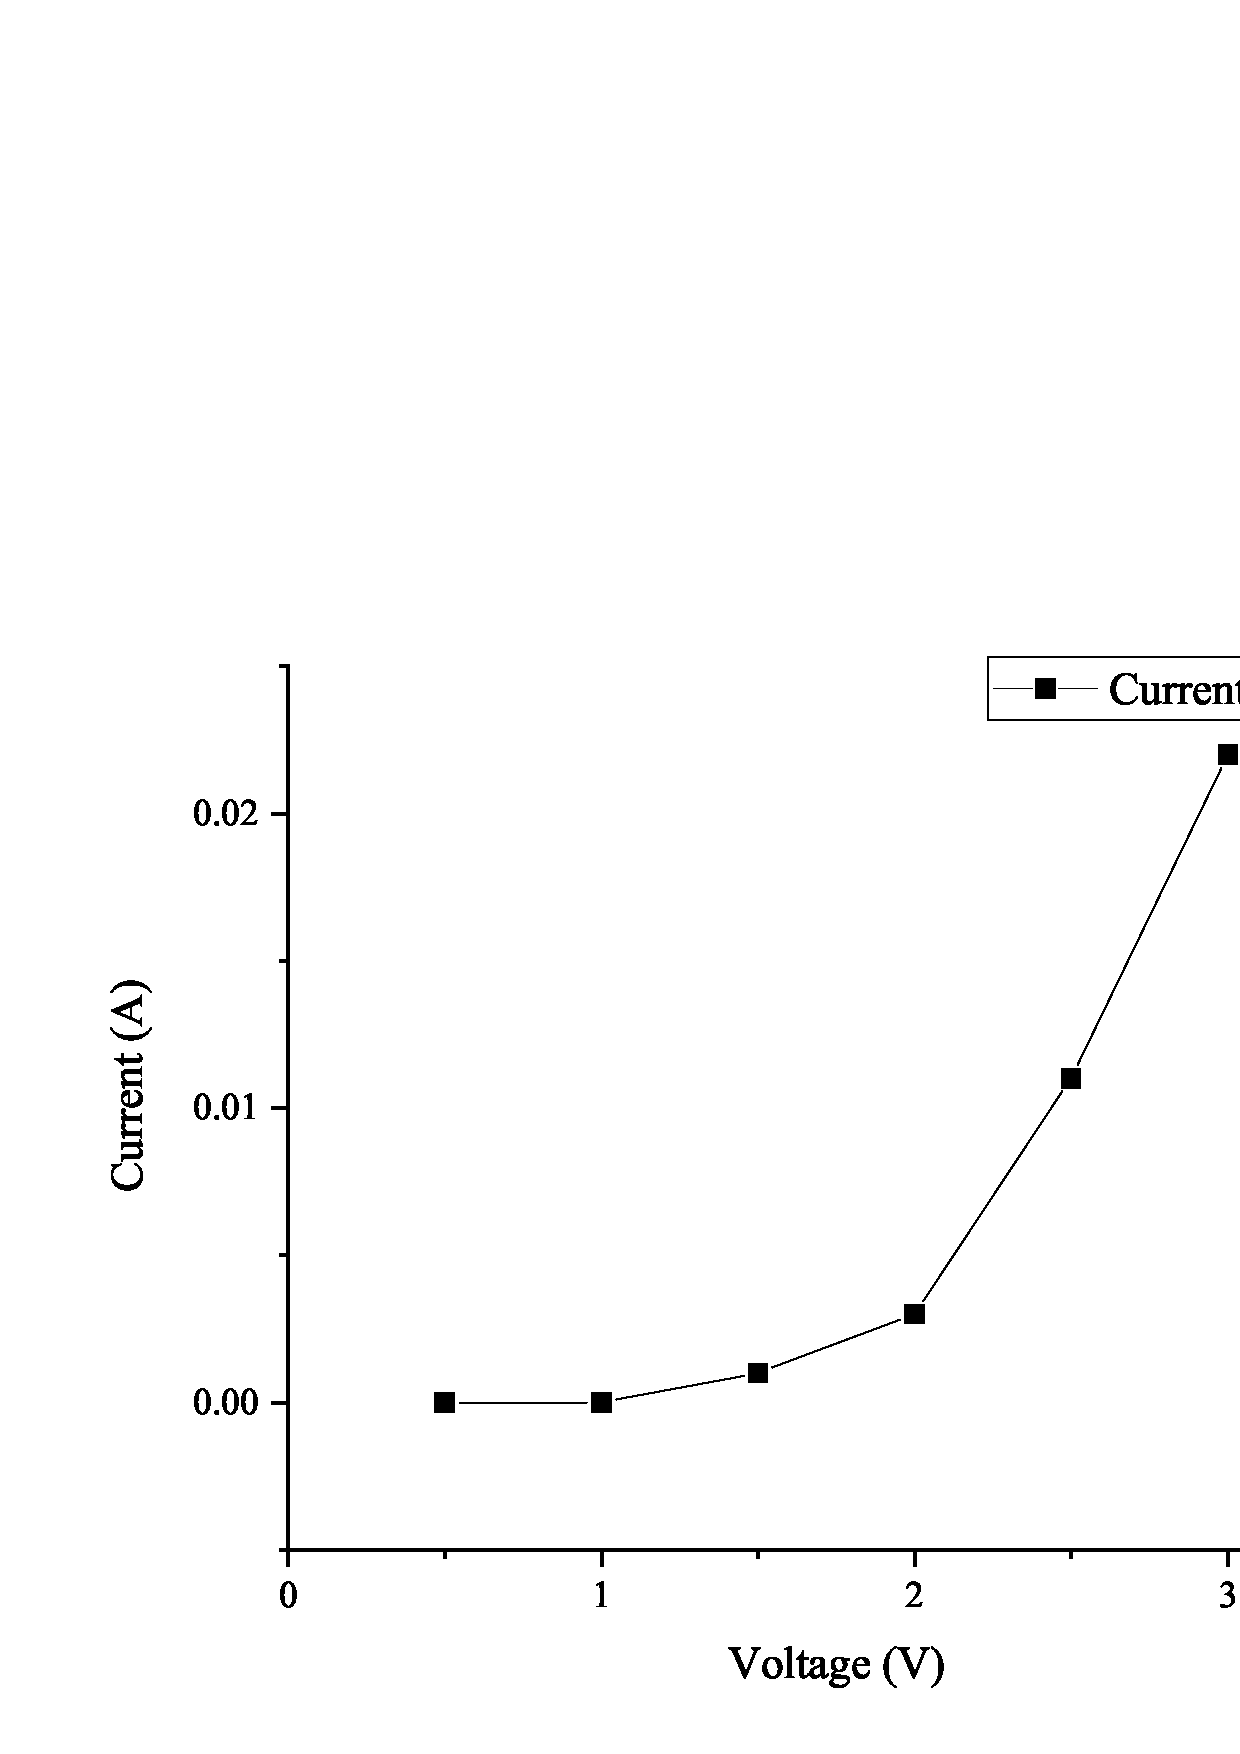
\includegraphics[width=0.8\linewidth]{7.jpg}
\end{figure}
\begin{figure}[H]
	\centering
	\includegraphics[width=0.8\linewidth]{8.jpg}
\end{figure}
For the band-stop filter, $H(\omega)=\frac{V_{out}(\omega)}{V_{in}(\omega)}=\frac{j(\omega L-\frac{1}{\omega C})}{R+j(\omega L-\frac{1}{\omega C})}$.

Note that $H(0)=0$, $H(\infty)=0$. The band-stop filter rejects a band of frequencies centered on the center frequency $\omega_0$, which is given by $\omega_0=1/\sqrt{LC}$.
\section{Measurement}
\begin{enumerate}[1.]
	\item According to the pre-lab assignments, we are supposed to fill in the Expected Data columns in the tables below before the lab.
	\item During the lab:
	\begin{enumerate}[i)]
		\item Construct the circuit for each type of filter. Resister: R = 982$\Omega$; Capacitor: C = 0.1$\mu$F; Inductor: L = 1mH.
		\item Set the Input Signal in the function generator to be Sine Wave with amplitude of 5 $\rm{V_{ppk}}$ and change the frequency accordingly.
		\item Use the oscilloscope to detect the amplitudes of the Input and Output signals. Record them respectively in the first two column in the tables.
		\item Additionally for the Band-reject Filter, when the frequency approach the critical frequency at which the Transfer Function Magnitude reaches its minimum, the Output Signal Amplitude changes rapidly. For a more accurate result, you can (but not strictly required to) add some more rows to record the data (Table V).
	\end{enumerate}
	\item After the lab, we should calculate with the experimental data for the "Transfer function magnitude" and "Transfer function magnitude, in dB" columns.
\end{enumerate}
\section{Results and Calculations}
\subsection{Low-pass Filter}
\begin{table}[H]
	\centering
	\begin{tabular}{|l|l|l|l|l|l|l|}
	\hline
	Frequency&\makecell[l]{Input\\signal\\amplitude,\\Vppk}&\makecell[l]{Output\\signal\\amplitude,\\Vppk}&\makecell[l]{Transfer\\function\\magnitude}&\makecell[l]{Expected\\transfer\\function\\magnitude}&\makecell[l]{Transfer\\function\\magnitude,\\in dB}&\makecell[l]{Expected\\transfer\\function\\magnitude,\\in dB}\\
	\hline
	1MHz&5.000&0.096&0.0192&0.0016&-34.33&-55.81\\
	\hline
	100kHz&5.000&0.125&0.0250&0.0162&-32.04&-35.81\\
	\hline
	50kHz&5.000&0.233&0.0466&0.0324&-26.63&-29.79\\
	\hline
	10kHz&5.000&1.09&0.2180&0.1600&-13.23&-15.92\\
	\hline
	5kHz&5.000&1.93&0.3860&0.3083&-8.268&-10.22\\
	\hline
	1kHz&5.000&4.6&0.9200&0.8510&-0.7242&-1.401\\
	\hline
	500Hz&5.000&5.0&1.0000&0.9556&0.0000&-0.3948\\
	\hline
	\end{tabular}
	\caption{Measurement data for low-pass filter.}
\end{table}

\begin{figure}[H]
	\centering
	\includegraphics[width=0.8\linewidth]{9.jpg}
	\caption{Measurement of low-pass filter.}
\end{figure}
\subsection{High-pass Filter}
\begin{table}[H]
	\centering
	\begin{tabular}{|l|l|l|l|l|l|l|}
	\hline
	Frequency&\makecell[l]{Input\\signal\\amplitude,\\Vppk}&\makecell[l]{Output\\signal\\amplitude,\\Vppk}&\makecell[l]{Transfer\\function\\magnitude}&\makecell[l]{Expected\\transfer\\function\\magnitude}&\makecell[l]{Transfer\\function\\magnitude,\\in dB}&\makecell[l]{Expected\\transfer\\function\\magnitude,\\in dB}\\
	\hline
	1MHz&5.000&5.0&1.0000&1.0000&0.0000&-1.141$\times10^{-5}$\\
	\hline
	100kHz&5.000&5.0&1.0000&0.9999&0.0000&-0.001141\\
	\hline
	50kHz&5.000&4.9&0.9800&0.9995&-0.1755&-0.004561\\
	\hline
	10kHz&5.000&4.8&0.9600&0.9871&-0.3546&-0.1126\\
	\hline
	5kHz&5.000&4.6&0.9200&0.9513&-0.7242&-0.4339\\
	\hline
	1kHz&5.000&2.21&0.4420&0.5251&-7.092&-5.595\\
	\hline
	500Hz&5.000&1.23&0.2460&0.2948&-12.18&-10.61\\
	\hline
	100Hz&5.000&0.281&0.0562&0.0616&-25.01&-24.21\\
	\hline
	\end{tabular}
	\caption{Measurement data for high-pass filter.}
\end{table}

\begin{figure}[H]
	\centering
	\includegraphics[width=0.8\linewidth]{10.jpg}
	\caption{Measurement of high-pass filter.}
\end{figure}
\subsection{Band-pass Filter}
\begin{table}[H]
	\centering
	\begin{tabular}{|l|l|l|l|l|l|l|}
	\hline
	Frequency&\makecell[l]{Input\\signal\\amplitude,\\Vppk}&\makecell[l]{Output\\signal\\amplitude,\\Vppk}&\makecell[l]{Transfer\\function\\magnitude}&\makecell[l]{Expected\\transfer\\function\\magnitude}&\makecell[l]{Transfer\\function\\magnitude,\\in dB}&\makecell[l]{Expected\\transfer\\function\\magnitude,\\in dB}\\
	\hline
	1MHz&5.000&0.54&0.1080&0.1545&-19.33&-16.22\\
	\hline
	500kHz&5.000&1.47&0.2940&0.2986&-10.63&-10.50\\
	\hline
	100kHz&5.000&4.3&0.8600&0.8485&-1.310&-1.427\\
	\hline
	50kHz&5.000&4.7&0.9400&0.9611&-0.5374&-0.3449\\
	\hline
	10kHz&5.000&4.9&0.9800&0.9952&-0.1755&-0.04159\\
	\hline
	1kHz&5.000&2.21&0.4420&0.5266&-7.092&-5.570\\
	\hline
	500Hz&5.000&1.23&0.2460&0.2951&-12.18&-10.60\\
	\hline
	\end{tabular}
	\caption{Measurement data for band-pass filter.}
\end{table}

\begin{figure}[H]
	\centering
	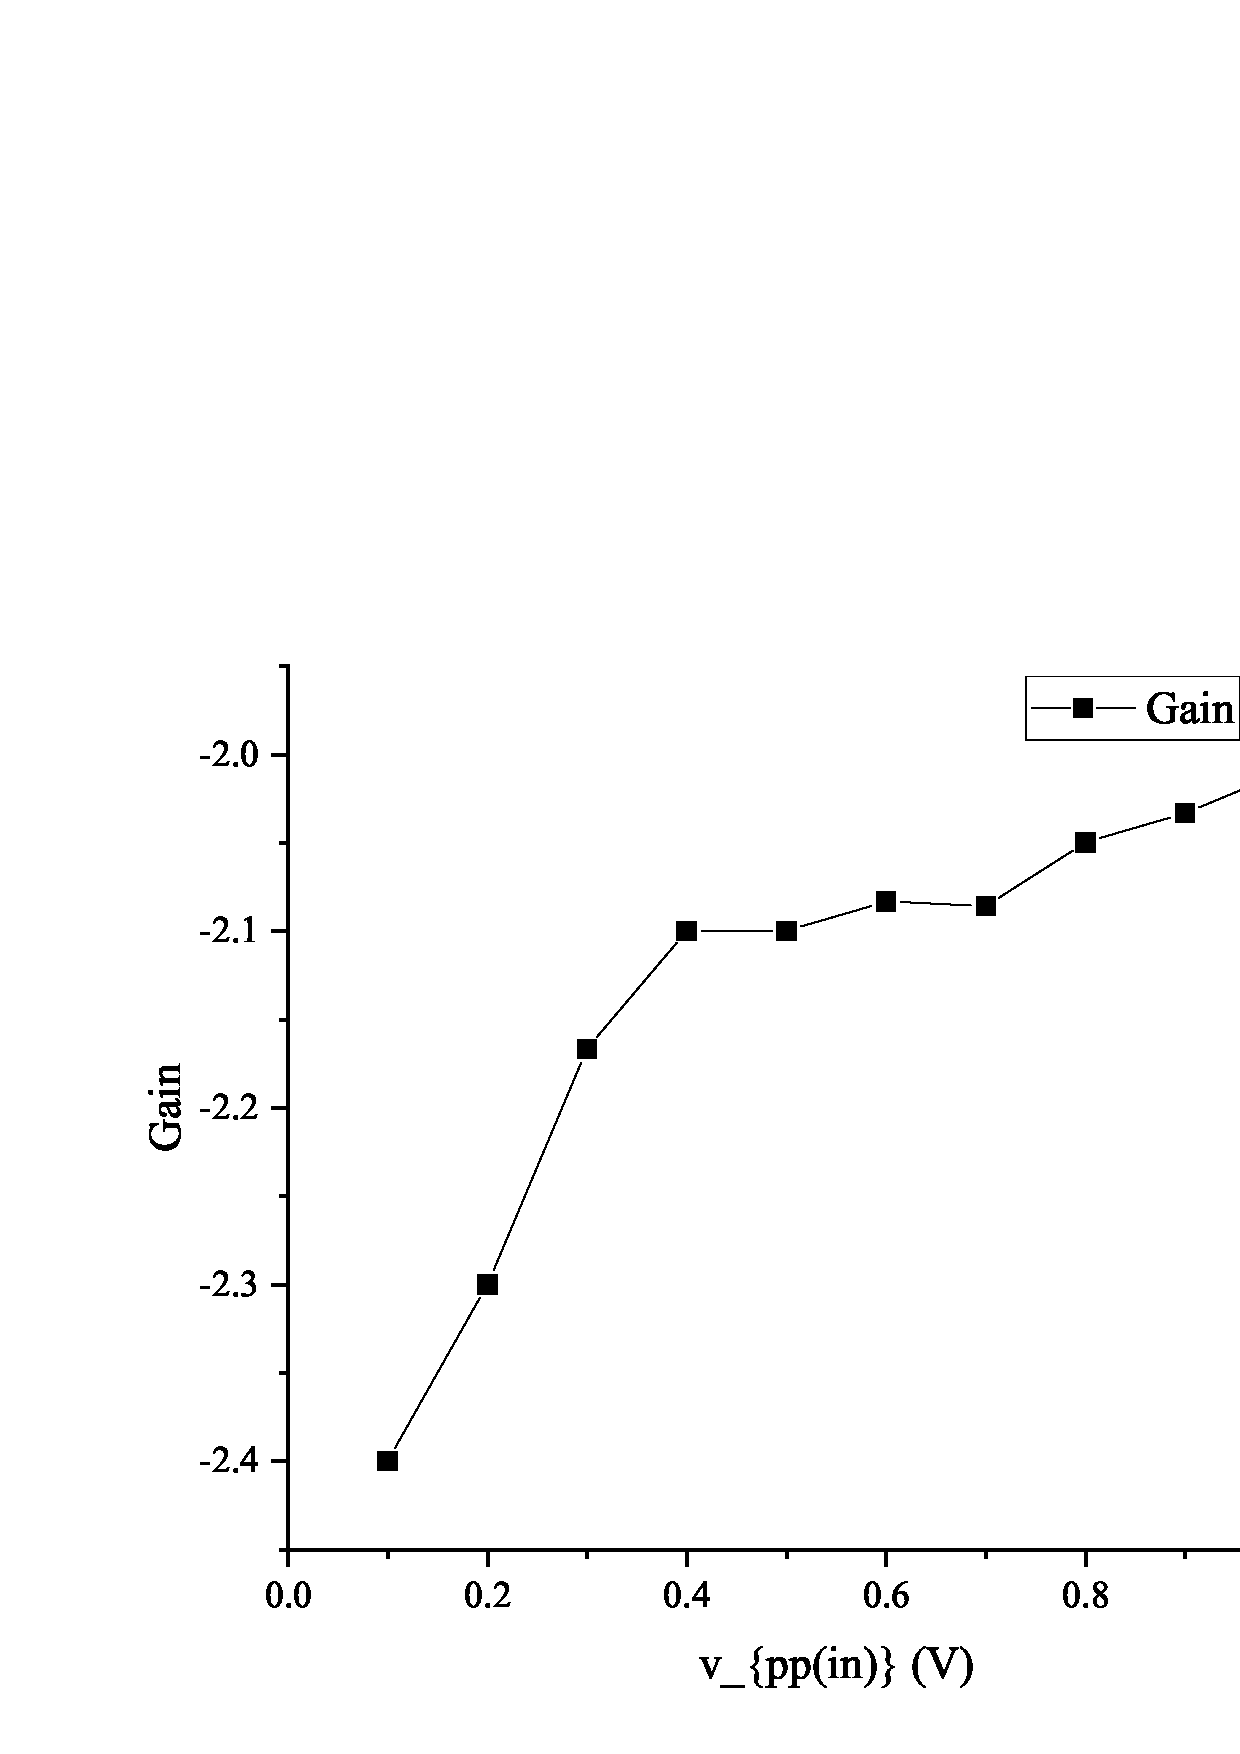
\includegraphics[width=0.8\linewidth]{11.jpg}
	\caption{Measurement of band-pass filter.}
\end{figure}
\subsection{Band-reject Filter}
\begin{table}[H]
	\centering
	\begin{tabular}{|l|l|l|l|l|l|l|}
	\hline
	Frequency&\makecell[l]{Input\\signal\\amplitude,\\Vppk}&\makecell[l]{Output\\signal\\amplitude,\\Vppk}&\makecell[l]{Transfer\\function\\magnitude}&\makecell[l]{Expected\\transfer\\function\\magnitude}&\makecell[l]{Transfer\\function\\magnitude,\\in dB}&\makecell[l]{Expected\\transfer\\function\\magnitude,\\in dB}\\
	\hline
	1MHz&5.000&5.2&1.0400&0.9880&0.3407&-0.1049\\
	\hline
	500kHz&5.000&5.1&1.0200&0.9544&0.1720&-0.4056\\
	\hline
	300kHz&5.000&4.7&0.9400&0.8863&-0.5374&-1.048\\
	\hline
	200kHz&5.000&4.1&0.8200&0.7860&-1.724&-2.091\\
	\hline
	100kHz&5.000&2.61&0.5220&0.5292&-5.647&-5.528\\
	\hline
	50kHz&5.000&1.31&0.2620&0.2763&-11.63&-11.17\\
	\hline
	10kHz&5.000&0.73&0.1460&0.0976&-16.71&-20.21\\
	\hline
	5kHz&5.000&1.79&0.3580&0.2804&-8.922&-11.04\\
	\hline
	1kHz&5.000&4.7&0.9400&0.8501&-0.5374&-1.410\\
	\hline
	500Hz&5.000&5.1&1.0200&0.9555&0.1720&-0.3956\\
	\hline
	\end{tabular}
	\caption{Measurement data for band-reject filter.}
\end{table}

\begin{figure}[H]
	\centering
	\includegraphics[width=0.8\linewidth]{12.jpg}
	\caption{Measurement of band-reject filter.}
\end{figure}
\section{Conclusion and Discussion}
In this experiment, in general, we obtained reasonable data for output signal amplitude in $\rm{V_{ppk}}$ and see that the trend of the transfer function magnitude follows the trend of the ratio of the output signal amplitude to the input signal amplitude.

However, when we measurement the output signal amplitude of band-reject filter, 3 of the digits have higher value than 5.0, i.e. the input signal amplitude. This error may come from the error of input signal amplitude, which possibly higher than $5.000\rm{V_{ppk}}$. Besides, the cursor is automatically generated by the oscilloscope without additional adjustment, which might be not accurate.

In conclusion, we learned about transfer functions and four types of filters – Low-Pass, High-Pass, Band-Pass, and Band-reject. Besides, We predicted the theoretical result of transfer function magnitude and made comparison with measurement data in lab.
\section*{Reference}
Lab 5 Manual.
\vspace{2cm}
\section*{Data sheet}
\newpage
\begin{figure}[H]
	\centering
	\includegraphics[width=1\linewidth]{13.jpg}
\end{figure}
\begin{figure}[H]
	\centering
	\includegraphics[width=1\linewidth]{14.jpg}
\end{figure}
\begin{figure}[H]
	\centering
	\includegraphics[width=1\linewidth]{15.jpg}
\end{figure}
\end{document}